%% LyX 2.0.5.1 created this file.  For more info, see http://www.lyx.org/.
%% Do not edit unless you really know what you are doing.
\documentclass[useAMS,usenatbib,letterpaper]{mn2e} 
\usepackage[totalwidth=480pt,totalheight=680pt,layoutvoffset=0.5cm]{geometry}
%\documentclass[usenatbib]{article}
\usepackage[latin9]{inputenc}
\geometry{verbose}
\usepackage{color}
\usepackage{float}
\usepackage{url}
\usepackage{amsmath}
\usepackage{amssymb}
\usepackage{astrobib_mnras2e}
\usepackage{graphicx}
\usepackage{times} 
\usepackage{fixltx2e}

\makeatletter

%%%%%%%%%%%%%%%%%%%%%%%%%%%%%% LyX specific LaTeX commands.
%% A simple dot to overcome graphicx limitations
\newcommand{\lyxdot}{.}


%%%%%%%%%%%%%%%%%%%%%%%%%%%%%% User specified LaTeX commands.
\newcommand{\mvir}{M_{\rm vir}}
\newcommand{\mcoll}{M_{\ast}}
\newcommand{\rvir}{R_{\rm vir}}
\newcommand{\vmax}{V_{\rm max}}
\newcommand{\meanvmax}{\overline{V}_{\rm max}}

\newcommand{\ximm}{\xi_{\rm mm}}
\newcommand{\xihm}{\xi_{\rm hm}}
\newcommand{\bh}{b_{\rm h}}
\newcommand{\bhlin}{b^{\rm lin}_{\rm h}}

%%% UNITS %%%
\newcommand{\msun}{M_{\odot}/h}
\newcommand{\mpch}{{\rm Mpc}/h}
\newcommand{\kpch}{{\rm kpc}/h}

%%%%%%%%%%%%%%%%%%%%%%%%%%%%%% LyX specific LaTeX commands.
%% A simple dot to overcome graphicx limitations
%Make my life significantly easier
\global\long\def\bd{{\bm{\delta}}}

\makeatother

\begin{document}

\title{The Maximum Circular Velocity Dependence of Halo Clustering}
\maketitle
\begin{abstract}
We study how the two-point clustering of dark matter halos depends on halo mass, $\mvir,$ and the depth of the gravitational potential well, $\vmax.$  At the low-mass end, halos with high-$\vmax$ show stronger large-scale clustering relative to halos with low-$\vmax$ of the same mass.  In keeping with previous results, this trend weakens and reverses for $\mvir>\mcoll\approx10^{12.5}\msun,$ such that large-scale bias is mildly stronger for low-$\vmax$ halos relative to their high-$\vmax$ counterparts. We present the first study of the scale-dependence of halo assembly bias. At the low-mass end, assembly bias exhibits a pronounced scale-dependent ``bump''  at $500\kpch-5\mpch,$ a new result. This feature weakens and eventually vanishes for halos of higher mass. We show that halo assembly bias can primarily be attributed to a special subpopulation of {\em ejected subhalos}, defined as present-day host halos that were previously members of a higher-mass halo at some point in their past history. Our findings have important implications for both cosmological parameter inference and galaxy evolution modeling. We find that predictions for galaxy clustering and lensing in the $r\sim1-2\mpch$ regime can be impacted by up to $\sim20\%$ by the choice of the halo property, even for stellar mass-limited samples. We conclude by outlining a program to alleviate this threatening systematic, so that existing and near-future surveys can achieve their promise to robustly constrain cosmology and the galaxy-halo connection using high-precision measurements of clustering and lensing. 

%At constant halo mass, we see residual dependence of halo clustering on $V_{{\rm max}}$. In low mass regime, high-$V_{{\rm max}}$ halos cluster more strongly than low-$V_{{\rm max}}$ halos; at $M_{{\rm vir}}\thickapprox10^{11.6}h^{-1}{\rm M_{\odot}}$, the linear bias for high-$V_{{\rm max}}$ halos is $40\%$ larger. In high mass regime, this trend reverses that low-$V_{{\rm max}}$halos cluster more strongly, and the overall difference is smaller. At $r<10h^{-1}{\rm Mpc}$, halo bias for high-$V_{{\rm max}}$ halos exhibit significantly different scale-dependent feature compared to the bias for low-$V_{{\rm max}}$ halos; high-$V_{{\rm max}}$ halos cluster strongly at $1h^{-1}{\rm Mpc}$ and their clustering signal differs by 60\% at $M_{{\rm vir}}\approx10^{11.8}h^{-1}{\rm M_{\odot}}$ compared to their low-$V_{{\rm max}}$counterparts. This scale-dependent feature, however, is significantly reduced by excluding ejected halos from the samples. The ejected halos are the halos which are identified as host halos at present epoch but were subhalos of more massive host halos in the past, and they are known to host satellite galaxies instead of central galaxies. As possible observational consequences of the results, we relate an observable property of a galaxy (luminosity, stellar mass) to an intrinsic property of its host halo (mass, circular velocity). By using different choices for the halo property, we see a clear scale dependence in clustering at $1h^{-1}{\rm Mpc}$, with a maximum difference of $\sim15\%$. These differences go down to $\sim5\%$ after removing the ejected halos.
\end{abstract}

\section{Introduction}

The halo model \citep[][for a recent review]{seljak00,vdboschBOOK} 
provides a connection between dark
matter halos and galaxies, and it has been remarkably successful in
describing observations of galaxy clustering. In particular, the
Halo Occupation Distribution (HOD) and the Conditional Luminosity
Function (CLF) are the two most widely used models of the galaxy-halo
connection. These models start from the assumption that halo mass completely determines
the galaxy occupation statistics. In order to populate halos with
galaxies, the HOD specifies the probability $P(N|M)$ that a halo with
mass $\mbox{M}$ hosts $N$ galaxies, while the CLF models the mean
abundance $\Phi(L|M)$ of galaxies with luminosity $L$ in halos of  mass $M$.
These two models are interchangeable; integrating the CLF over luminosity
yields an HOD. Both models have been applied
extensively to observations in order to study the halo-galaxy connection
\citep{magliocchetti03,zehavi05a,yang_etal05,zheng07,vdBosch07,zheng09,skibba09,simon_etal09,ross10,zehavi11,geach12,parejko13}
as well as cosmology \citep{tinker05,leauthaud11b,more_etal13,cacciato_etal13,mandelbaum13}.

However, the clustering of halos also exhibits a
dependence on additional properties beyond their mass 
\citep{gao_etal05,wechsler06,gao_white07,li_etal08}, a
phenomenon generically referred to as halo assembly bias. This can be 
traced back to the fact that halos of
the same mass in different environments have different assembly histories
and cluster differently. Having different assembly histories also affects
the internal structure of halos. This, in turn, results in a clustering dependence
on the structural properties of a halo, including the depth of its 
gravitational potential well, characterized by its maximum circular
velocity $V_{\rm max}$. This work revisits this manifestation 
of halo assembly bias, and extends it down to smaller scales ($< 10 h^{-1} {\rm Mpc}$) 
than has been previously explored.

An alternative approach to connecting halos and galaxies is abundance
matching
\citep{kravtsov04a,vale_ostriker04,tasitsiomi_etal04,vale_ostriker06,conroy_wechsler09,
guo10,simha10,neistein11a,watson_etal12b,rod_puebla12,kravtsov13}. 
In its simplest form, abundance matching posits a monotonic
relationship between a property of a galaxy (luminosity, stellar mass) 
and that of a halo (mass, potential well depth). By construction, 
such a relationship preserves the rank ordering of the galaxies and halos. 
The choice of this halo property is a priori unknown. In light of 
the previous discussion of assembly bias, one would naturally 
expect this choice to affect the predicted clustering properties 
of halos. This work aims to quantify these differences, again
focusing on smaller scales than previous studies.

%%As a response to halo assembly bias, a recent trend in connecting
%%halos and galaxies has been to use the Abundance Matching technique
%%\citep{kravtsov04a,vale_ostriker04,tasitsiomi_etal04,vale_ostriker06,conroy_wechsler09,
%%guo10,simha10,neistein11a,watson_etal12b,rod_puebla12,kravtsov13},
%%which assumes a monotonic relation in size of galaxies and halos in
%%order to assign galaxies to halos in a hierarchical manner. In order
%%to evaluate size of halos, the maximum circular velocity, which is
%%a measure of potential well depth of halos, is often used due to its
%%tight correlation with stellar mass of galaxies. In the Abundance
%%Matching technique, halo assembly bias is a generic prediction.

A recent parallel research effort has been revisiting the standard
subdivision of dark matter halos into host/sub-halos, which depends
on how the halo boundary is chosen. While the virial radius is the
most commonly chosen definition, recent work has demonstrated that the
environmental effects of halos extends well beyond the virial radius
\citep{wetzel_etal13, diemer14,adhikari14,wetzel_nagai14,more15}. 
In particular, \cite{wetzel_etal13} argue that these environmental effects
are due to ejected subhalos which orbit beyond the virial radius
of their hosts, and therefore get temporarily reclassified as host
halos. These studies 
argue that a more physically motivated boundary is the 
``splashback radius'' corresponding to the caustic from material 
just reaching its first apocentric passage. This work demonstrates
that the halo assembly bias on small scales predominantly 
arises from this mis-classification.

The outline of this paper is as follows. Sec.~2 summarizes the simulations
we use in this work. Sec.~3 presents our primary results - characterizing
the dependence of the clustering of halos on $V_{\rm max}$; Sec.~4 explores
some of the implications of these results. We conclude in Sec.~???.

%%%Besides halo assembly bias, there have been several studies discussing
%%%definition of a more physically motivated boundary for halos. A virial
%%%radius of halos is commonly used as a boundary definition. Those studies,
%%%however, show that halos and their environmental effects extend well
%%%beyond the virial radius and a more physically motivated boundary
%%%is a ``splashback'' radius at which splashback material generates
%%%a caustic \citep{diemer14,adhikari14,wetzel_nagai14,more15}.
%%%The environmental effects of halos beyond their virial radius is also
%%%found in galaxy groups and clusters; galaxies which are beyond the
%%%virial radius of groups/clusters tend to have more quiescent star
%%%formation rates \cite{wetzel_etal13}. \cite{wetzel_etal13}
%%%shows that it is due to ejected satellite galaxies which orbit beyond
%%%their host halo's virial radius and eventually fall back in. Those
%%%ejected satellite galaxies live in ejected halos, which were within
%%%the virial radius of more massive host halos in the past but identified
%%%as a distinguished halo at present epoch. Since those ejected halos
%%%host very different type of galaxies than central galaxies that host
%%%halos host, it is crucial to understand the effect of ejected halos
%%%on halo clustering.

%%In this paper, we explore the additional dependence of galaxy clustering
%%on the central velocity dispersion both on small and large scales.
%%In Section 2, we briefly describe the simulations, halo finding algorithm,
%%and identification of halo types. In Section 3, we explore halo clustering
%%as a function of halo mass and the maximum circular velocity through
%%two-point correlation functions. We also investigate the effect of
%%ejected halos on the halo clustering. In Section4, we show how the
%%Abundance Matching techniques based on halo mass and the maximum circular
%%velocity make qualitatively different predictions for the clustering
%%of central galaxies to connect our findings in Section 3 to observations.
%%In Section 5, we discuss the implications of our results and summarize
%%our main conclusions.
%%

\section{Simulations}

\textbf{NP : Check the mass limits}

We use the Bolshoi \citep{bolshoi_11} and Multidark simulations \citep{riebe_etal11, prada_etal11}
\footnote{\url{http://www.multidark.org}%
} in this work; the combination of these simulations allows us to span
a large range in halo mass. We summarize key properties of these simulations
here. Both simulations were run with the Adaptive Refinement Tree
Code \citep{kravtsov_etal97,gottloeber_klypin08} assuming a flat
$\Lambda{\rm CDM}$ model with density parameters $\Omega_{m}=0.27$,
$\Omega_{\Lambda}=0.73$, $\Omega_{b}=0.0469$, and $\sigma_{8}=0.82$,
$n=0.95$, $h=0.70$. The Bolshoi simulation used $2048^{3}$ particles
in a $250h^{-1}{\rm Mpc}$ box and a force resolution of $1h^{-1}{\rm kpc}$,
giving a particle mass of $1.35\times10^{8}h^{-1}{\rm M_{\odot}}$,
while the Multidark simulation used $2048^{3}$ particles in a $1h^{-1}{\rm Gpc}$
box and a force resolution of $7h^{-1}{\rm kpc}$ giving a particle
mass of $8.721\times10^{9}h^{-1}{\rm M_{\odot}}$. Dark matter halos
and subhalos are identified using the \texttt{ROCKSTAR} phase-space,
temporal halo finder \citep{rockstar} and merger trees are constructed
using the \texttt{CONSISTENT TREES} \citep{rockstar_trees} procedures%
\footnote{The catalogues used in this paper are publicly available at \url{http://hipacc.ucsc.edu/Bolshoi/MergerTrees.html}%
}. All of the results we consider here are at $z=0$.

In what follows, we use the virial masses and maximum circular velocities
(tagged ``\texttt{mvir}'' and ``\texttt{vmax}'') directly from
the halo catalogues. The halo mass and velocity functions start to
show incompleteness at $10^{11}h^{-1}M_{\odot}$ ($\sim740$ particles)
for the Bolshoi simulation, and $10^{12}h^{-1}M_{\odot}$ ($\sim100$
particles) for the Multidark simulation. We choose to be conservative
and restrict to halos with $>740$ particles for both simulations,
corresponding to mass limits of $10^{11}h^{-1}{\rm M_{\odot}}$ and
$6.45\times10^{12}h^{-1}{\rm M_{\odot}}$ for Bolshoi and Multidark
respectively.

In addition to the standard classification of halos into host halos
(not within the virial radius of a more massive halo) and subhalos
(within the virial radius of a more massive halo), we further classify
host halos into ejected and non-ejected halos. Ejected halos, also
referred to as ``backsplash'' halos, are host halos whose main progenitor
was classified, at some point in its merger tree history, as a subhalo.
As we discuss below, these ejected halos have very different clustering
properties compared to their non-ejected counterparts. The ejected
fraction for the Bolshoi simulation is $\sim15.8\%$ at $10^{11}h^{-1}M_{\odot}$,
and drops to $\sim6.3\%$ at $10^{13}h^{-1}M_{\odot}$. The lower
mass resolution of the Multidark simulation prevents us from making
this additional sub-classification. Accordingly, results that rely
on this split are restricted to the Bolshoi simulation and mass range.


\section{The Maximum Circular Velocity Dependence of Halo Clustering}

In this section we present our primary results. We begin in \S\ref{subsec:samples}
by describing the sample of halos we use throughout the paper, as
well as our method for how we categorize halos as having above- or
below-average circular velocities for their mass. In \S\ref{subsec:halobias}
...


\subsection{Halo Sample Definitions}

\label{subsec:samples}

If the internal structure of a dark matter halo of mass $\mvir$ is
described by an NFW profile \citep{nfw97} of concentration $c,$
then its maximum circular velocity $\vmax$ is given by: 
\begin{equation}
\overline{V}_{{\rm max}}=0.465M_{{\rm vir}}^{1/3}\sqrt{G(\frac{4}{3}\pi\Delta_{{\rm h}}\rho_{{\rm crit}}\Omega_{m})^{1/3}\frac{c}{{\rm ln(1+c)-c/(1+c)}}}.\label{eq:vmax-mvir}
\end{equation}
As shown in \citep{klypin10a}, the median concentration-mass relation
$\bar{c}(\mvir)$ for $z=0$ Bolshoi halos is well-described by: 
\begin{equation}
{\rm log}_{10}\bar{c}=-0.097{\rm log_{10}M_{vir}}+2.148.\label{eq:concen}
\end{equation}
For every halo in the Bolshoi and Multidark catalogs, we use its tabulated
$\mvir$ to compute $\bar{c}(\mvir),$ and then use the values $\bar{c}$
together with Eq.~\ref{eq:vmax-mvir} to compute $\overline{V}_{{\rm max}}$
for every halo. We will henceforth refer to halos with $\vmax<\meanvmax(\mvir)$
as ``low-$\vmax$ halos'', and halos with $\vmax>\meanvmax(\mvir)$
as ``high-$\vmax$ halos''. Thus a halo's high- or low-$\vmax$
designation refers to whether its true $\vmax$ value in the simulation
is above- or below-average for its mass.

\begin{figure}
\begin{center}
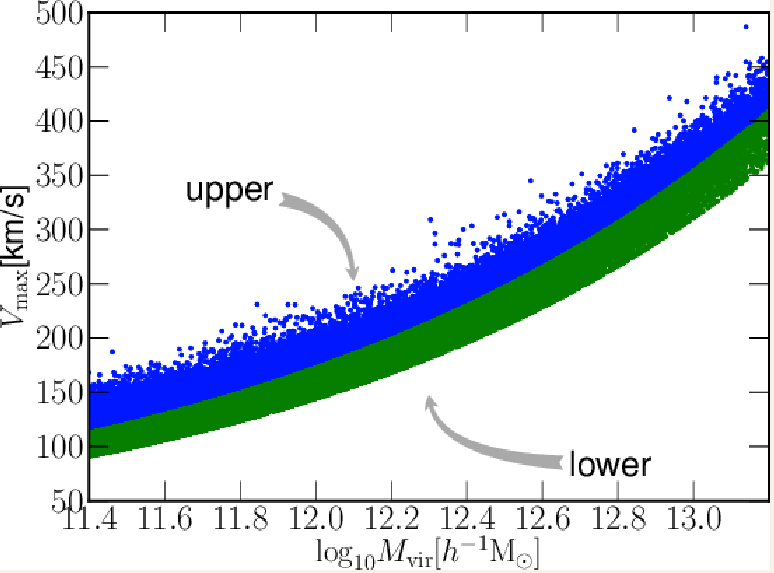
\includegraphics[width=0.9\columnwidth]{../plots/plaecholder}
\end{center}
\caption{\label{fig:vmax-mvir}Distribution of halo mass and maximum circular
velocity at $z=0.0$ for halos\textcolor{black}{{} from the Bolshoi
simulation.} The blue dots represent halos whose observed maximum
circular velocity, $V_{{\rm max,obs}}$, is greater than $\overline{V}_{{\rm max}}$,
while the green dots are the ones with smaller $V_{{\rm max,obs}}$
than $\overline{V}_{{\rm max}}$. The boundary between blue and green
dots correspond to $\overline{V}_{{\rm max}}$ computed from Eq. \ref{eq:vmax-mvir}.}
\end{figure}


%%% APH: Discussion of binning is not necessary for Figure 1, is it?


Fig. \ref{fig:vmax-mvir} illustrates the distribution of Bolshoi
halos as a function of $\mvir$ and $\vmax.$ High-$\vmax$ halos
are shown in blue, low-$\vmax$ halos in green. The dividing line
between the two samples is defined by Eq.~\ref{eq:vmax-mvir}. We
find that our analytical approximation for $\meanvmax(\mvir)$ gives
a good description of the true median: for any fixed value of $\mvir,$
the high-$\vmax$ and low-$\vmax$ subsamples have very similar numbers
of objects.

Note that Fig. \ref{fig:vmax-mvir} shows a sharp lower bound on the
value of $\vmax$ at a given $\mvir,$ but no sharp upper bound. This
is ultimately due to the halo mass definition. The circular velocity
$V_{{\rm cir}}$ at the virial radius of any halo is $V_{{\rm cir}}(\rvir)\equiv V_{{\rm vir}}=\sqrt{G\mvir/\rvir}.$
Since the value of $\vmax$ tabulated in the halo catalog is computed
as the maximum value of $V_{{\rm cir}}$ over the entire profile of
the halo, formally $\vmax$ cannot exceed $V_{{\rm vir}}.$ This manifests
as the sharp lower bound seen in Fig. \ref{fig:vmax-mvir}.


\subsection{Halo Bias}

\label{subsec:halobias}

In this section we present our primary results for the clustering
properties of halos as a function of $\mvir$ and $\vmax.$ Clustering
strength is quantified by the two-point correlation function, $\xi(r).$
In all that follows, we will use $\ximm(r)$ to denote the auto-correlation
of the dark matter density field with itself, and $\xihm(r)$ to denote
the cross-correlation between a sample of halos and the underlying
density field.

Halos are biased tracers of the dark matter density field. We denote
this bias as $\bh,$ which is in general a function of spatial separation.
We define halo bias as 
\[
\bh(r)\equiv\xihm(r)/\ximm(r).
\]
On sufficiently large scales halo bias is approximately linear, and
$\bh(r)$ approaches a constant value $\bhlin.$

In order to measure the bias of a sample of simulated halos, for both
Bolshoi and Multidark we estimate $\ximm(r)$ and $\xihm(r)$ using
a random down-sampling of $10^{6}$ dark matter particles. For a given
sample of halos, we estimate the value of $\bhlin$ exhibited by the
sample as follows: 
\begin{equation}
b_{{\rm lin}}=\sum_{i}(\xi_{hm}(r_{i})/\xi_{mm}(r_{i}))/N_{{\rm bin}}.\label{eq:blindef}
\end{equation}
In Eq.~\ref{eq:blindef}, the sum is performed over $N_{{\rm bin}}=20$
separation bins $r_{{\rm i}}$ linearly spaced from $10h^{-1}{\rm Mpc}$
to $20h^{-1}{\rm Mpc}.$

In order to study the mass-dependence of halo bias, we bin our halos
into a sequence of $\mvir$ bins chosen such that there are the same
numbers of halos in each bin. For Multidark, we select $2\times10^{5}$
halos for each bin; for Bolshoi we use $25000$ halos per bin. The
halos in each mass bin are categorized as high-$\vmax$ or low-$\vmax$
according to the method described in \S\ref{subsec:samples}. We
start using halos from the Multidark simulation for $M_{{\rm vir}}>10^{12.3}h^{-1}{\rm M_{\odot}}$. 

The top panel of Fig.~\ref{fig:linear-bias} shows $\bhlin$ as a
function of $\mvir;$ results for high-$\vmax$ halos are shown in
blue, low-$\vmax$ halos in green. At the low-mass end, linear bias
is a weak function of $\mvir;$ for $\mvir\gtrsim10^{13}\msun$ we
see that $\bhlin$ increases sharply with $\mvir.$ Thus the basic
shape of each curve in Fig. \ref{fig:linear-bias} is in accord with
theoretical expectations from the peak-background split \citep{sheth_tormen99}
formalism and Press-Schechter theory \citep{pressschechter74}.

By comparing the blue and green curves in Fig.~\ref{fig:linear-bias}
we can see that linear bias has significant dependence upon $\vmax$
for halos of the same mass. This dependence is most readily seen in
the bottom panel, which shows the ratio of $\bhlin$ of high-$\vmax$
samples divided by $\bhlin$ of low-$\vmax$ samples. Thus in the
bottom panel of Fig.~\ref{fig:linear-bias}, vertical axis values
exceeding unity correspond to masses where high-$\vmax$ halos cluster
more strongly relative to their low-$\vmax$ counterparts.

At the low-mass end, high-$\vmax$ halos are more strongly clustered
than low-$\vmax$ halos of the same mass. The clustering difference
increases with decreasing $\mvir,$ and exceeds $30\%$ for halos
of Milky Way mass $\mvir\approx10^{12}\msun.$ At the high-mass end,
the trend reverses, and the overall magnitude is weaker. These results
are consistent with \citet{wechsler06}, who find that the same trends
hold when the secondary halo property is NFW concentration, rather
than $\vmax.$ This agreement is to be expected: insofar as the halo
profile is well-approximated by an NFW profile, $\vmax$ is entirely
determined by concentration (see Eq.~\ref{eq:vmax-mvir}).

\begin{figure}
\begin{center}
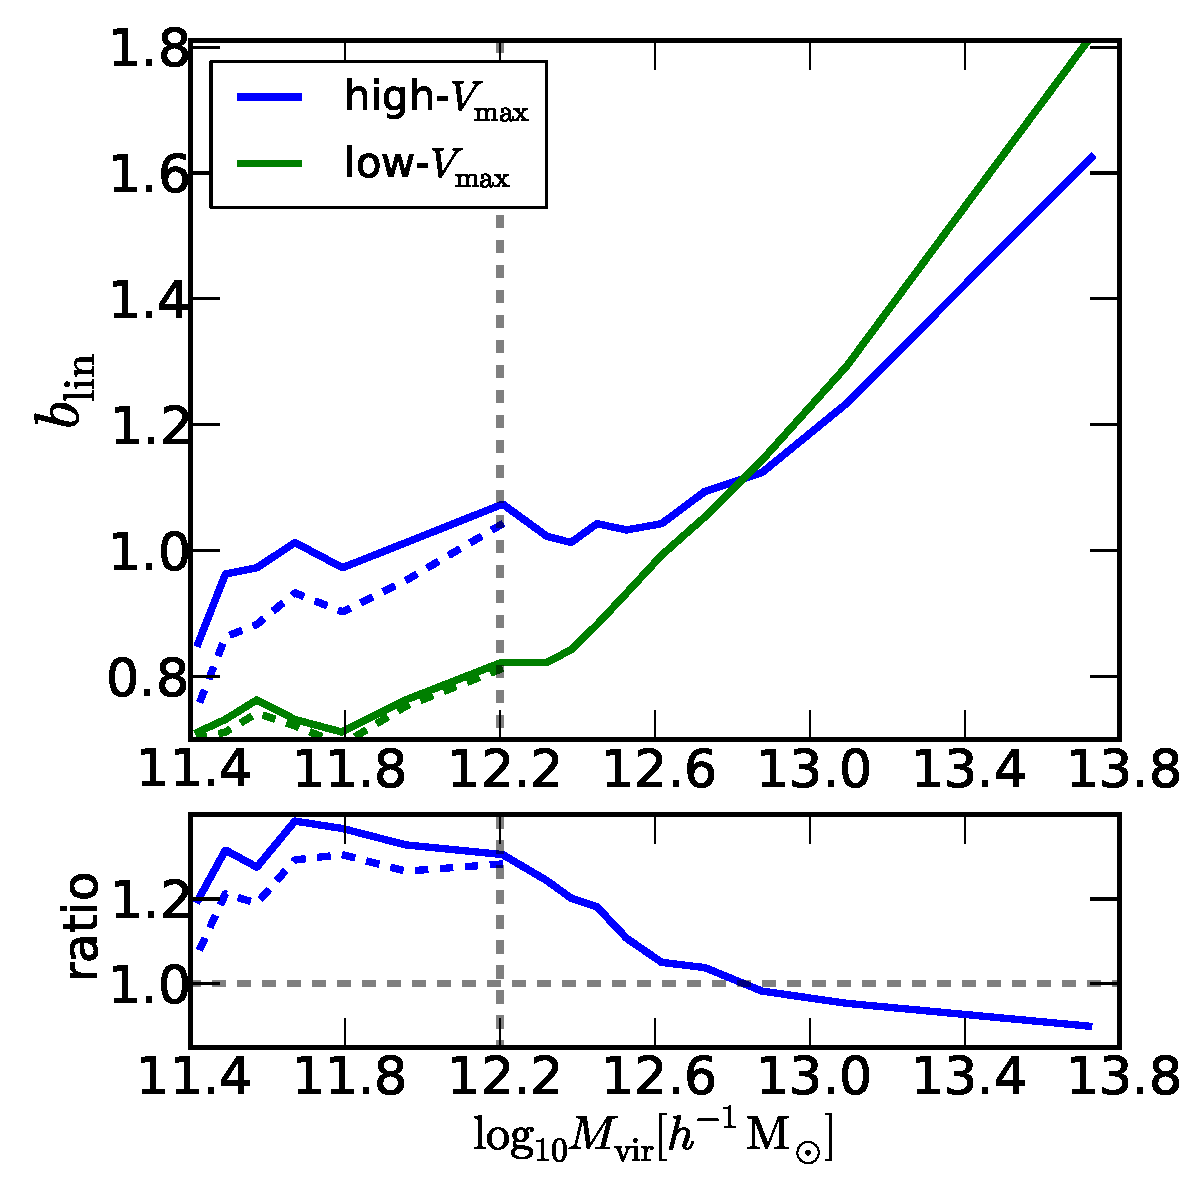
\includegraphics[width=0.9\columnwidth]{../plots/linearBias_wang}
\end{center}
\caption{\label{fig:linear-bias}Upper panel: Linear bias at $z=0.0$ as a
function of halo mass from the Bolshoi simulation (circle points)
and the MultiDark simulation (triangle points). The blue circles correspond
to a linear bias for high-$V_{{\rm max}}$ halos, while the green
circles correspond to low-$V_{{\rm max}}$ halos. Lower panel: Ratio
of linear biases between high-$V_{{\rm max}}$ and low-$V_{{\rm max}}$
samples from the Bolshoi simulation and the MultiDark simulation.
The clustering difference increases with decreasing $\mvir,$ and
exceeds $30\%$ for halos of Milky Way mass $\mvir\approx10^{12}\msun.$}
\end{figure}


Next, we study scale-dependence of halo bias on small scales for high-$V_{{\rm max}}$
and low-$V_{{\rm max}}$ halos. Fig. \ref{fig:small-scale} shows
the ratio of halo bias $b_{h}(r)$ of high-$V_{{\rm max}}$ samples
divided by $b_{h}(r)$ of low-$V_{{\rm max}}$ samples for several
mass bins. The first three mass bins labeled in the figure, ${\rm log_{10}M[h^{-1}{\rm M_{\odot}}]=11.7,12.0,12.2}$,
are from the Bolshoi simulation, and the last two mass bins, ${\rm log_{10}M[h^{-1}{\rm M_{\odot}}]=12.7,13.1}$,
are from the MultiDark simulation. The ratio is normalized by their
linear biases so that the ratio goes to 1 on large scales. High-$V_{{\rm max}}$
halos cluster more strongly compared to their low-$V_{{\rm max}}$
counterparts at $1h^{-1}{\rm Mpc}$. This scale-dependent feature
becomes stronger with decreasing $M_{{\rm vir}}$ and exceeds 40\%
for halos of Milky Way mass and reaches 60\% at $M_{{\rm vir}}\approx10^{11.7}h^{-1}{\rm M_{\odot}}$.

Up until present, we have used both host halos and ejected halos to
compute halo biases. Both types of halos are identified as distinct
halos at $z=0$. Ejected halos, however, are halos which were identified
as part of more massive halos at one or more occasions in the past,
but were ejected and now exist at a host halo at $z=0$. Those ejected
halos tend to exist around more massive halos (any reference?). Therefore,
the effect on scale-dependent biases may be caused by those ejected
halos. To test this, we compute halo-matter cross correlation functions
without the ejected halos. Similar to Fig. \ref{fig:linear-bias},
we first compare linear biases as a function of halo mass. The ratio
of linear bias between high-$V_{{\rm max}}$ and low-$V_{{\rm max}}$
halos is suppressed to 25\% for halos of Milky Way mass. Similar to
what was done in Fig. \ref{fig:small-scale}, Fig. \ref{fig:eject}
shows the ratio of $b_{h}(r)$ between high-$V_{{\rm max}}$and low-$V_{{\rm max}}$
halos on small scales for several mass bins only from the Bolshoi
simulation. Due to the mass resolution of the Multidark simulation,
we do not have sufficient number of ejected halos in the halo catalog.\textcolor{black}{{}
Once the ejected halos have been removed, the deviation of the halo
bias on small scales is greatly reduced. }This implies an intimate
connection between assembly bias and subhalo back-splashing. 

This scale dependence in the clustering signal from ejected halos
has a very simple interpretation. By definition, ejected halos are
physically associated with a more massive halo. Their clustering signal
is therefore determined by this associated halo, much like the clustering
of subhalos is determined by its host halo. More quantitatively, \cite{wetzel_etal13}
find the fraction of ejected halos is a strong function of the corresponding
host halo mass. For $10^{11.7}h^{-1}M_{\odot}$ halos, the host halos
are predominantly $>10^{14}h^{-1}M_{\odot}$ and their spatial distribution
peaks at roughly the virial radius (Figs. 2 and 3 in \cite{wetzel_etal13}).
This is broadly consistent with our results, where we find the strongest
scale dependence at $1h^{-1}{\rm Mpc}$.

\begin{figure}
\begin{center}
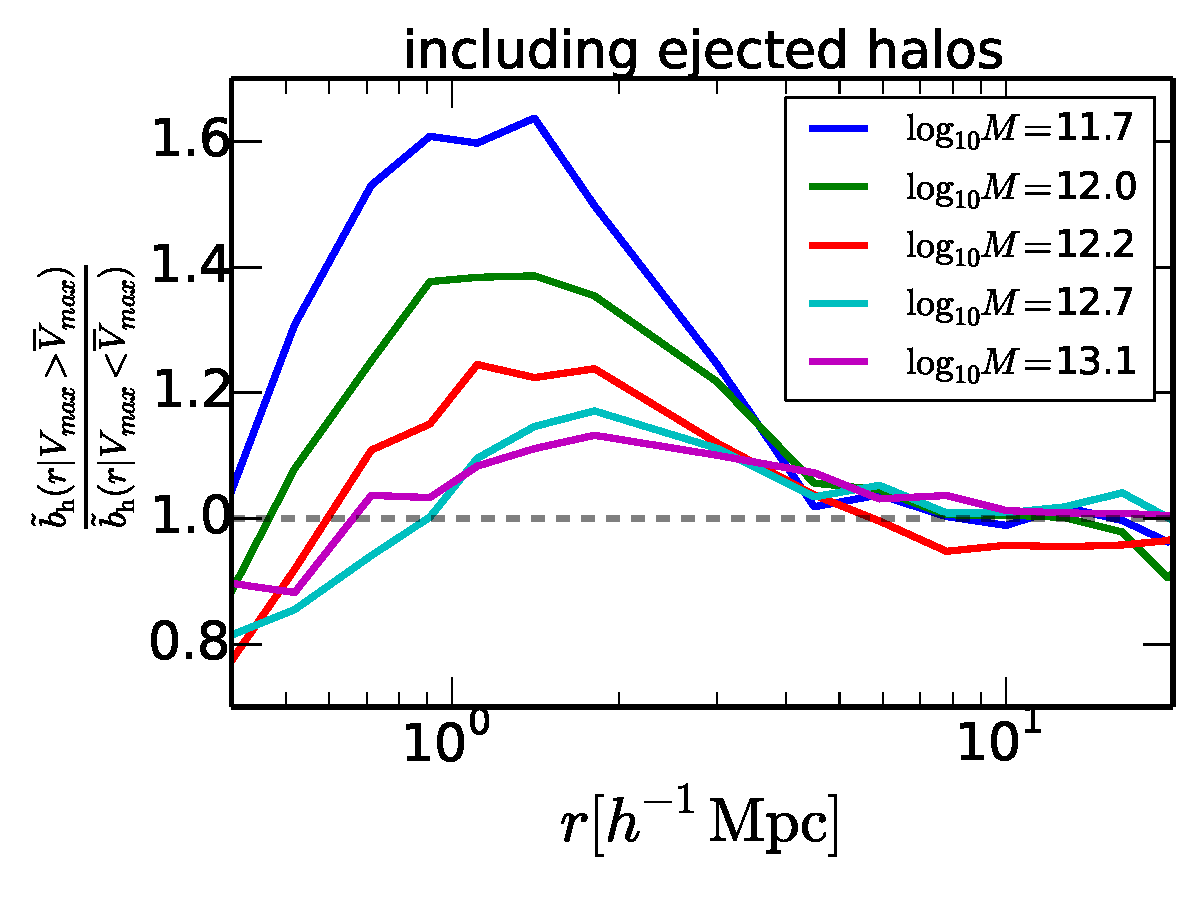
\includegraphics[width=0.9\columnwidth]{../plots/Both_smallScale_wang_log}
\end{center}
\caption{\label{fig:small-scale}Ratio of halo-matter cross correlation functions
between high/low-$V_{{\rm max}}$ halos normalized by their linear
biases. The plots are from the Bolshoi simulation and the MultiDark
simulation at $z=0$. Each line corresponds to different halo mass
bins labeled in the plots. The top three lines that correspond to
low mass halos are computed from halos in the Bolshoi simulation,
while the bottom lines are from the MultiDark simulation. Those plots
show that high-$V_{{\rm max}}$ halos cluster more strongly than low-$V_{{\rm max}}$
halos at $1h^{-1}{\rm Mpc}$ and the relative scale-dependence between
those subsamples increases smoothly with decreasing halo mass. }
\end{figure}


\begin{figure}
  \begin{center}
  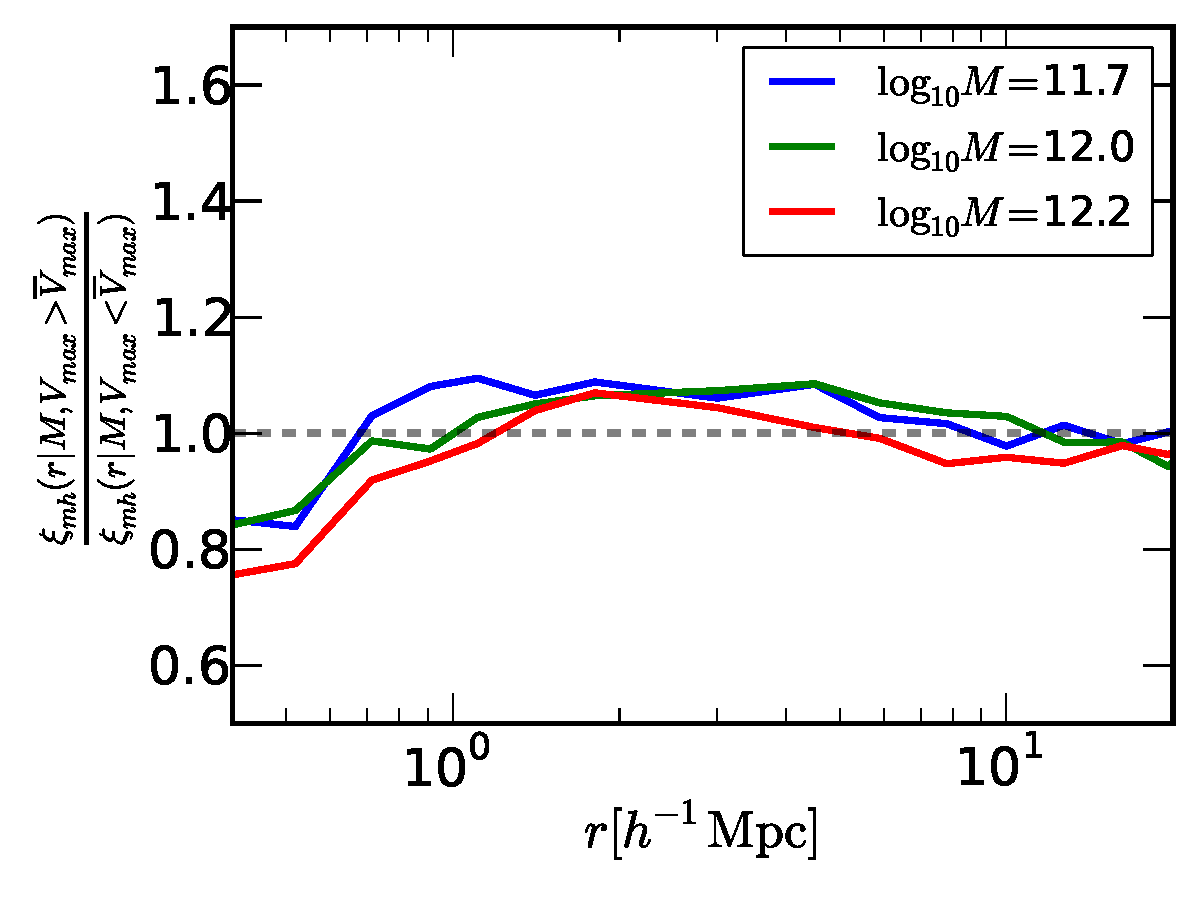
\includegraphics[width=0.9\columnwidth]{../plots/Bolshoi_smallScale_wang_log_eje}
\end{center}
\caption{\label{fig:eject}The same figures as Fig. \ref{fig:small-scale}
without ejected halos only from the Bolshoi simulation. As can be
seen by comparing these results to those in Fig. \ref{fig:small-scale},
the $V_{{\rm max}}$-dependence of halo bias on small scales is dramatically
reduced by excluding ejected subhalos. This implies an intimate connection
between assembly bias and subhalo back-splashing.}
\end{figure}



\section{Observational Consequences}

\textbf{NP : Probably should explicitly show that the mean halo masses
of these samples is the same}

We now consider possible observational consequences of the results
of the previous section. In order to do this, the key first step is
to relate an observable property of a galaxy (luminosity, stellar
mass) to an intrinsic property of its host halo (mass, circular velocity).
As one might infer from above (and we demonstrate below), different
choices for the latter can result in significant differences for different
observables.

In order to be explicit, we consider abundance matching (CITE??) the
stellar masses of central galaxies to either the mass or circular
velocity of host halos. We implement this by splitting the halo catalog
into a series of bins with constant number density (=$1.6\times10^{-3}$),
rank ordering either by mass or circular velocity. We label each bin
by its corresponding stellar mass, computed from the stellar-to-halo
mass relation of CITE Behroozi et al. When we rank order based on
circular velocity, there is the possibility that the effective halo
masses of these bins could differ from what we obtain after rank ordering
by halo mass. We explicitly check this and find that the effective
halo masses for both cases agree to $\sim0.4\%$, allowing us to consistently
compare samples with the same imputed stellar mass.

At fixed stellar mass, the linear bias of samples selected by their
circular velocity are $\sim5\%$ higher than samples selected by halo
mass. This decreases to $\sim2\%$ if we remove ejected halos from
both samples. Fig.~\ref{fig:abundance_small} shows the ratio of
the small scale ($1$ to $10h^{-1}{\rm Mpc}$) correlation functions
of these two samples, both including {[}left{]} and excluding {[}right{]}
ejected subhalos. As previously, we see a clear scale dependence of
this signal, with a maximum difference of $\sim15\%$ at $\sim1h^{-1}{\rm Mpc}$.
These differences go down to $\sim5\%$ after removing ejected subhalos.

{\bf NP : Missing figure here}
\begin{figure}
\begin{center}
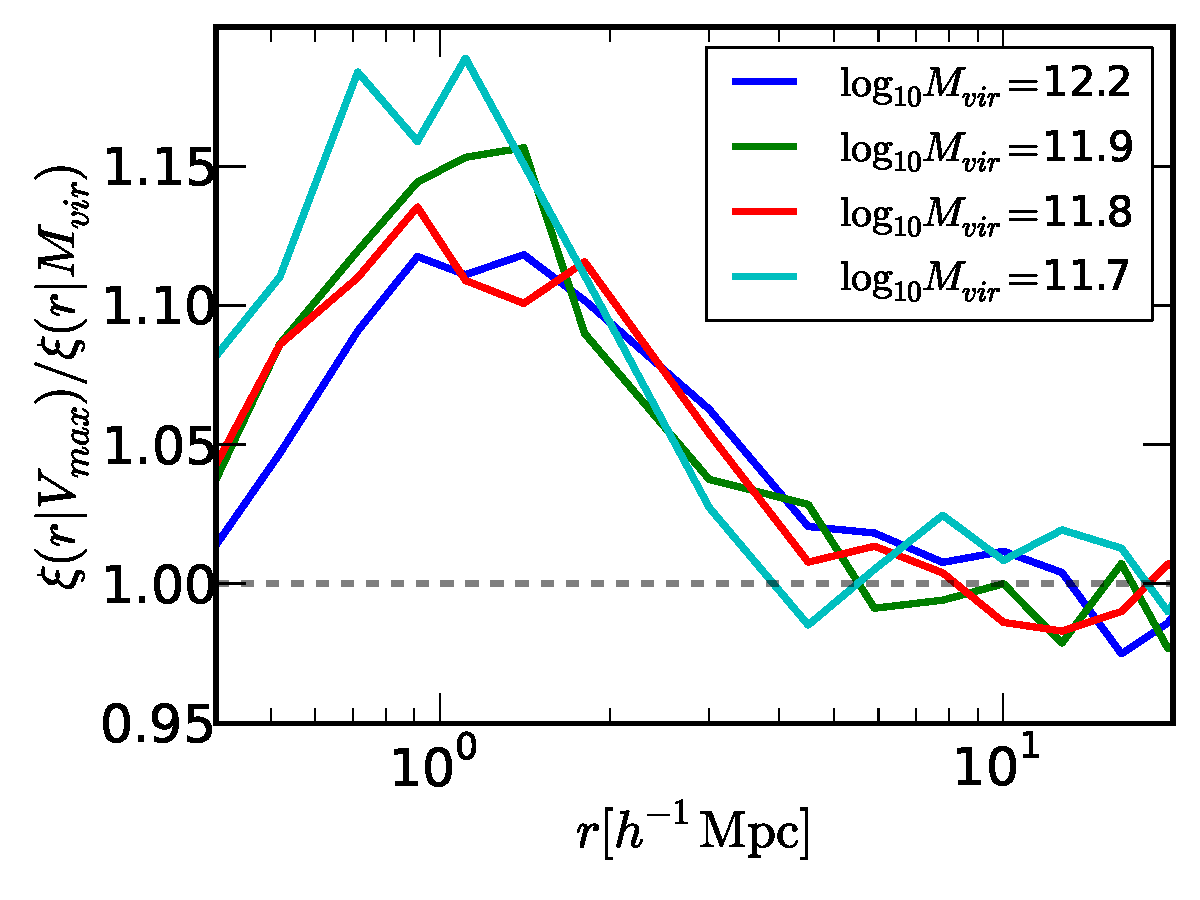
\includegraphics[width=0.9\columnwidth]{../plots/Bolshoi_andrew_smallScale}
%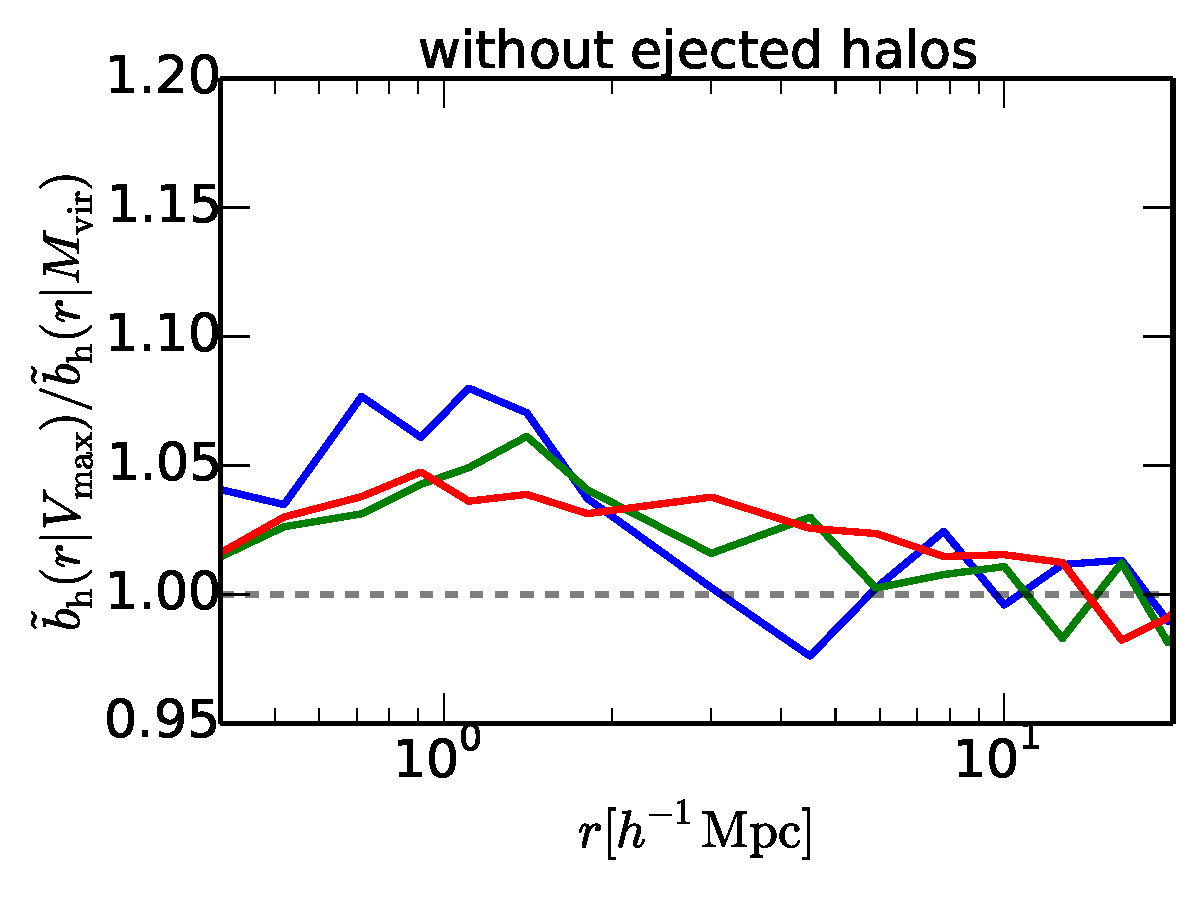
\includegraphics[width=0.9\columnwidth]{../plots/Bolshoi_andrew_smallScale_nonEj}
\end{center}
\caption{\label{fig:abundance_small}Ratio of halo-matter cross correlation
functions between$M_{{\rm vir}}$-based and $V_{{\rm max}}$-based
abundance matching samples with ejected halos (left) and without ejected
halos (right). The ratios are normalized by their linear biases. Each
line corresponds to different halo mass bins labeled in the plots.
With ejected halos, the halo biases computed from the $V_{{\rm max}}$-samples
have very different scale-dependence than the ones from the $M_{{\rm vir}}$-samples.
By removing those ejected halos, the difference is more or less removed.}
\end{figure}



\subsection{$\Delta\Sigma(r)$}

--Select a bin of Milky Way mass host halos, and select their number-density-matched
Vmax-selected equivalent. Use Peter Behroozi's stellar-to-halo mass
relation to estimate the stellar mass of the central galaxy that would
be found in these halos, then plot the halo-matter cross-correlation
as a function of scale, over-plotting the two results.

--want to show: We show that the galaxy-galaxy lensing signal of low-mass
centrals is impacted at the xxx-yyy\% level, in a highly scale-dependent
fashion, by the theoretical choice to empirically connect stellar
mass to either host halo Vmax or Mvir.


\section{Discussion}

% I really like the organization of this Discussion. I have kept it as is, and just provided more flesh to your existing text, which was quite well-written. 

%%% I've added a Summary section so that we can avoid having to repeat ourselves so much in the Discussion
%In this paper, we explore additional dependence of halo clustering on the maximum circular velocity of halos in addition to halo mass. The maximum circular velocity is a measure of potential well depth of halos, which determines the escape velocity of particles around the halos and therefore determines the feedback efficiency for galaxy formation.

For halos $M_{{\rm vir}}\gtrsim\mcoll\approx10^{12.5}\msun,$ we have shown that the linear bias of low-$V_{{\rm max}}$ halos 
is larger relative to high-$V_{{\rm max}}$ halos of the same mass. As shown in \citet{dalal_etal08}, this 
phenomenon is nicely explained in terms of the statistics of fluctuations in a Gaussian random field.
Consider two halos with the same present-day mass, but with different concentration. Both halos originate from a 
 fluctuation of the same peak height, but with different peak curvature: the high-concentration (high-$\vmax$) halo 
has a sharper peak than the low-concentration (low-$\vmax$) halo. 
\citet{dalal_etal08} showed that a generic prediction of Extended Press Schechter theory (EPS) with a configuration space filter 
is that low-curvature peaks cluster more strongly relative to high-curvature peaks of the same height. In closely related work, 
 \citet{zentner07} used EPS with a configuration space filter to show that for a pair of halos of the same peak height, the early-forming halo should 
 reside in a denser large-scale environment than the late-forming one.\footnote{See Chapter IX, Section D.}

A critical assumption underlying these EPS predictions is that a halo is the dominant peak in its large-scale environment. This is a well-founded assumption at the high-mass end, and we see that the predictions are in good agreement with simulations in the $\mvir>\mcoll$ regime \citep{dalal_etal08}. The situation is quite different when $\mvir\lesssim\mcoll.$ We have confirmed previous results \citep[e.g.,][]{wechsler06} that assembly bias changes sign and strengthens for lower-mass halos. This is in stark contrast to the EPS model described above, which makes the same prediction for assembly bias regardless of halo mass. 

Thus EPS succeeds and fails in precisely the regimes where we expect. Lower-mass halos are strongly influenced by the tidal field in which they evolve \citep{hahn_etal07b,wang_etal11,shi15,hahn_etal09,hearin_etal15}; the EPS assumption that the halo dominates its environment breaks down catastrophically, and in this regime nonlinear evolution governs assembly bias. High-mass halos do dominate their tidal environment; the EPS assumption holds good, and we can understand assembly bias as naturally arising from the statistics of Gaussian fluctuations. 

Our results on the scale-dependence of assembly bias are also consistent with this picture. 
First, we remind the reader that halo bias for high-$\vmax$ halos
shows non-trivial scale dependence with a pronounced bump at $\sim1-2\mpch$
compared to the bias for low-$\vmax$ halos. This scale-dependent
feature for high-$\vmax$ halos becomes 60\% larger compared
to low-$\vmax$ halos at $M_{{\rm vir}}\approx10^{11.7}\msun$. 
This feature, however, is removed by excluding the ejected halos, 
implying that this special sub-population is responsible for the scale-dependent bump. 

Recent advances in our understanding of halo growth sheds light on the above results. 
As shown in \citet{diemer14,adhikari14,wetzel_nagai14,more15}, the natural physical boundary of a dark matter is the 
so-called ``splashback radius", which is the radius where accreted matter reaches its
first apocenter after turnaround, and is roughly $2-3\rvir.$ As shown in \citet{wetzel_etal13}, the $1-3\rvir$ region of the outskirts of 
halos of massive groups and clusters ($\mvir\gtrsim10^{13}\msun,$ $\rvir\gtrsim500\kpch$) is populated with 
a large fraction of ejected halos, which by definition are physically associated with the
more massive halo. The bump feature we find at $1-2\mpch$ is therefore at the same physical scale 
that we would expect if the clustering of the ejected population is largely 
determined by the host with to the halos are ultimately bound. 



%wang_mo_jing08 - need to cite


\textcolor{black}{In Section 4, we demonstrate that abundance matching
techniques, which relate an observable property of a galaxy (luminosity,
stellar mass) to an intrinsic property of its host halo (mass, circular
velocity), give a very different scale dependence on halo bias at
$r<10h^{-1}{\rm Mpc}$; we see a clear scale dependence in clustering
at $1h^{-1}{\rm Mpc}$, with a maximum difference of $\sim15\%$ with
the ejected halos and $\sim5\%$ without the ejected halos. Since
this scale-dependence correlates strongly with whether the host halo
samples selected by halo mass or maximum circular velocity, we can
possibly test whether a stellar mass of a galaxy is tightly correlated
with one of those two parameters in observations.}

In summary, we found a consistent trend with previous works in additional
dependence of linear bias on the maximum circular velocity for both
high/low mass halos. We also found that scale dependence of halo assembly
bias on small scales mostly come from the ejected halos.


\section{Summary}
\label{section:summary}

We conclude the paper with an overview of our primary results:

\begin{enumerate}
\item At fixed mass $\mvir,$ the large-scale bias of halos exhibits significant residual dependence on potential well depth $\vmax.$ At the low-mass end, high-$\vmax$ halos cluster more strongly than their low-$\vmax$ counterparts. At the high-mass end, this trend reverses, and is generally weaker, with the transition occurring at $\mcoll\approx10^{12.5}\msun.$ Our results are quantitatively consistent with previous studies of halo assembly bias. 
\item We show that assembly bias exhibits complex scale-dependence. The $\vmax-$dependence of halo clustering shows a pronounced ``bump" on scales $500\kpch\lesssim r\lesssim 5\mpch.$ This scale-dependence is itself mass-dependent: the bump feature is strongest for low-mass halos and vanishes for halos with $\mvir\gtrsim\mcoll.$
\item Assembly bias in both the linear and scale-dependent regimes can primarily be attributed to a special sub-population of {\em ejected subhalos}. If this special population is excluded from the halo sample, the strength of assembly bias is limited to $\lesssim5\%$ on all scales and for all masses $\mvir\gtrsim10^{11.75}\msun.$
\end{enumerate}















\bibliographystyle{mn2elong}
\bibliography{VmaxMvir}

\end{document}

